\subsection{Propagator interface}
\label{sec:system}

We now turn to the implementation of theory propagation in \clingo~5
and detail the structure of its interface depicted in Figure~\ref{fig:interface}.
%
\begin{figure}
  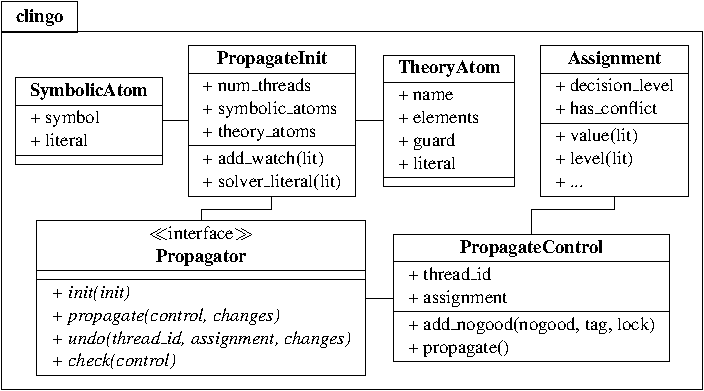
\includegraphics[width=\textwidth]{figures/python-interface}
  \caption{Class diagram of \clingo's (theory) propagator interface\label{fig:interface}}
\end{figure}
%
The interface \code{Propagator} has to be implemented by each custom propagator.
After registering such a propagator with \clingo,
its functions are called during initialization and search as indicated % in the algorithm
in Figure~\ref{fig:cdcl}.
%
Function \code{Propagator.init}%
\footnote{For brevity, we below drop the qualification \code{Propagator} and use its function names unqualified.}
is called once before solving (line~(\ref{fig:cdcl:init}) in Figure~\ref{fig:cdcl})
to allow for initializing data structures used during theory propagation.
It is invoked with a \code{PropagateInit} object providing access to symbolic (\code{SymbolicAtom}) as well as theory (\code{TheoryAtom}) atoms.
Both kinds of atoms are associated with program literals,\footnote{Program literals are also used in the \aspif\ format (see Appendix~\ref{sec:aspif}).} % ~\cite{gekakaosscwa16b}
which are in turn associated with solver literals.%
\footnote{Note that \clasp's preprocessor might associate a positive or even negative solver literal with multiple atoms.\label{fnt:solver:literals}}
Program as well as solver literals are identified by non-zero integers, where positive and negative numbers represent positive or  negative literals, respectively.
In order to get notified about assignment changes, a propagator can set up watches on solver literals during initialization.

During search, function \codeClass{Propagator}{propagate} is called with a \code{PropagateControl} object
and a (non-empty) list of watched literals that got assigned in the recent round of unit propagation (line~(\ref{fig:cdcl:propagate}) in Figure~\ref{fig:cdcl}).
The \code{PropagateControl} object can be used to inspect the current assignment, record nogoods, and trigger unit propagation.
Furthermore, to support multi-threaded solving,
its \code{thread\_id} property identifies the currently active thread,
each of which can be viewed as an independent instance of the CDCL algorithm in Figure~\ref{fig:cdcl}.%
%Hence, thread-specific state has to be associated with the \code{thread\_id}.
\footnote{%
Depending on the configuration of \clasp, threads can communicate with each other.
For example, some of the recorded nogoods can be shared.
This is transparent from the perspective of theory propagators.}
%
Function \codeClass{Propagator}{undo} is the counterpart of \codeClass{Propagator}{propagate}
and called whenever the solver retracts assignments to watched literals (line~(\ref{fig:cdcl:undo}) in Figure~\ref{fig:cdcl}).
In addition to the list of watched literals that have been retracted (in chronological order),
it receives the identifier and the assignment of the active thread.
%
Finally, function \codeClass{Propagator}{check} is similar to \codeClass{Propagator}{propagate},
yet invoked without a list of changes.
Instead, it is (only) called on total assignments
(line~(\ref{fig:cdcl:check}) in Figure~\ref{fig:cdcl}), independently of watches.
%
Overriding the empty default implementations of propagator methods is optional.
% Implementing the propagator methods, which default to empty implementations, is optional. % that does nothing.
For brevity, we below focus on implementations of the methods in \python,
while \C, \cpp, or \lua{} could be used as well.

%%% Local Variables:
%%% mode: latex
%%% TeX-master: "paper"
%%% End:
